% =============================================================================
% Nota de procedencia (no se imprime)
% Cifras primarias: reports/gbt_report_ladder500_imp_reconcile.json
%                   reports/gbt_summary_ladder500_imp_reconcile.md
%                   reports/scores_ladder500_imp_reconcile.npz
% Desplazamiento sellado: reports/reconcile_shift_protocol.json
% No usar reports/pitch_summary_bench500_pp.md: es un artefacto histórico.
% reports/benchmark_summary_bench500_imp.md corresponde a la ejecución principal.
% =============================================================================
\documentclass[11pt,a4paper]{article}

\usepackage[utf8]{inputenc}
\usepackage[T1]{fontenc}
\usepackage{lmodern}
\usepackage[spanish,es-tabla,es-noshorthands]{babel}
\usepackage[margin=2.5cm]{geometry}
\usepackage{amsmath,amssymb}
\usepackage{graphicx}
\usepackage{booktabs}
\usepackage{siunitx}
\usepackage{microtype}
\usepackage{authblk}
\usepackage[numbers,sort&compress]{natbib}
\usepackage[colorlinks=true,linkcolor=blue,citecolor=blue,urlcolor=blue]{hyperref}
\usepackage{setspace}
\usepackage{caption}
\usepackage{enumitem}
\usepackage{xcolor}

\graphicspath{{figures/}}

\newcommand{\todo}[1]{\textcolor{red}{[PENDIENTE: #1]}}
\setlength{\parskip}{0.4em}
\setlength{\parindent}{0pt}

\title{\textbf{Aprendizaje \emph{in silico} de la optimización AV/VV en TRC a partir de la impedancia intracardíaca}}

\author[1]{Lucas Costa\thanks{Autor corresponsal:
\texttt{2000.costalucas@gmail.com}.}}

\date{\today}

\begin{document}

\maketitle

\begin{abstract}
\noindent
\textbf{Antecedentes.} Cerca de un tercio de los pacientes que reciben terapia de
resincronización cardíaca (TRC) no responde al tratamiento. Diversos estudios han
señalado que los algoritmos automáticos de optimización AV/VV pueden superar a
los métodos clásicos basados en ECG solo en un pequeño subconjunto de pacientes;
en el resto, la eficacia es igual o menor. Recientemente, la Universidad de
Maastricht evaluó un enfoque basado en la detección de ruidos cardíacos mediante
un micrófono piezoeléctrico integrado en el marcapasos, que permitió estimar el
óptimo con una eficacia similar a la del ECG. Sin embargo, muchos pacientes no
pudieron beneficiarse de este método debido a la degradación de la señal causada
por el ruido del micrófono durante el movimiento corporal.
La impedancia intracardíaca ya se registra en la mayoría de los dispositivos de
TRC y se ha relacionado con la contractilidad ventricular; no obstante, se
desconoce si contiene información suficiente para un optimizador basado en datos.

\textbf{Objetivo.} Estimar, dentro de una simulación controlada, la utilidad de
la información proporcionada por la impedancia intracardíaca para optimizar los
ajustes AV y VV, y comparar modelos de ordenación lineales interpretables, de
conjuntos de árboles y de aprendizaje profundo bajo un desplazamiento sellado del
dominio del sensor.

\textbf{Métodos.} Se generaron 500 pacientes virtuales con el modelo CircAdapt
(VanOsta2024) y se realizaron barridos de 8 ajustes AV $\times$ 7 ajustes VV por
paciente (56 ajustes; 28\,000 observaciones etiquetadas). Se simularon tres
latidos por ajuste y se analizó el último, asumido en estado estacionario. Al
modelo de sensor se añadieron ganancia, desplazamiento de línea base, ruido y
deriva, de acuerdo con un modelo fenomenológico con dos dominios disjuntos. Se
extrajeron 42 características interpretables de impedancia, contexto y ajuste, y
la optimización se planteó como un problema de aprendizaje para ordenar
(\emph{learning-to-rank}). En particular, se compararon varios modelos: un modelo
de ordenación lineal por pares, LambdaMART, una CNN unidimensional pequeña,
variantes híbridas con \emph{embeddings} de la CNN y una mezcla de ordenaciones
ponderada por validación. Los modelos se entrenaron con 350 pacientes, se
validaron con 75 y se evaluaron en 75 pacientes reservados. La métrica de
evaluación fue la fracción de pacientes cuyo ajuste predicho no distaba más del
2\,\% del mejor trabajo sistólico; una tolerancia del 5\,\% constituyó el
criterio pragmático preespecificado. Se reservó como conjunto de prueba externa
un dominio de impedancia deliberadamente extremo y disjunto.

\textbf{Resultados.} El modelo de ordenación lineal seleccionó un ajuste casi
óptimo (dentro del 2\,\%) en el 64.0\,\% de los pacientes de prueba en el dominio
de origen (pérdida media 1.8\,\%) y en el 64.0\,\% bajo el desplazamiento del
sensor. Con la tolerancia del 5\,\%, estos valores fueron 88.0\,\% y 86.7\,\%.
El modelo de ordenación lineal combinado con los \emph{embeddings} de la CNN
alcanzó el 80.0\,\% al 2\,\% (pérdida 1.09\,\%) en el dominio de origen y el
94.7\,\% al 5\,\%; bajo el desplazamiento del sensor, los valores fueron
68.0\,\% al 2\,\% y 89.3\,\% al 5\,\%. Una mezcla ponderada por validación
seleccionó ese mismo modelo (80.0\,\%/68.0\,\% al 2\,\%;
94.7\,\%/89.3\,\% al 5\,\%). Un modelo sin características de la onda (contexto y
programación) alcanzó el 49.3\,\% al 2\,\% y el 68.0\,\% al 5\,\% en ambos
dominios, mientras que un control negativo con etiquetas permutadas se redujo al
8.0\,\%.

\textbf{Conclusiones.} La simulación indica que la impedancia intracardíaca
contiene información útil para los modelos de ordenación simples. A juicio del
autor, esto justificaría una prueba piloto con pacientes reales, dada la
facilidad para integrar el software en el hardware existente, que en general ya
registra la impedancia intracardíaca.
\end{abstract}

\vspace{0.5em}
\noindent\textbf{Palabras clave:} terapia de resincronización cardíaca;
impedancia intracardíaca; optimización AV y VV; learning-to-rank; aprendizaje automático; in silico; CircAdapt

% -----------------------------------------------------------------------------
\section{Introducción}
% -----------------------------------------------------------------------------

La terapia de resincronización cardíaca (TRC) reduce las tasas de hospitalización
y de mortalidad en pacientes seleccionados con insuficiencia cardíaca y
desincronización ventricular, pero las tasas de respuesta se mantienen en torno
al 70\,\%, de modo que aproximadamente un tercio de los pacientes no obtiene el
beneficio esperado. La programación de los retrasos auriculoventricular (AV) e
interventricular (VV) es uno de los determinantes modificables de la respuesta;
sin embargo, el óptimo es específico de cada paciente y cambia con el tiempo.
Además, existen factores predictores de la respuesta que pueden hacer
insuficiente el tratamiento habitual \citep{aalen2020}.

Los algoritmos existentes de optimización automática no han demostrado un
beneficio general frente a los métodos de ECG habitualmente utilizados
\citep{knijnik2023}, aunque sí en determinadas subpoblaciones. Por ejemplo, el
sensor de contractilidad SonR, que ajusta semanalmente los intervalos AV y VV, no
fue inferior a la optimización guiada por ecocardiografía y se asoció con una
tasa de hospitalizaciones por insuficiencia cardíaca un 35\,\% menor que la de
referencia, con una mayor tasa de respuesta en pacientes con fibrilación
auricular (FA) o insuficiencia renal (IR) \citep{brugada2016,singh2017}. Por otra
parte, la medición de ruidos cardíacos integrada en el dispositivo y combinada
con aprendizaje automático puede estimar el óptimo AV con una precisión
comparable a la de los métodos existentes; sin embargo, la señal se degrada
considerablemente por el movimiento y el ruido ambiental, de modo que un
subconjunto de pacientes no aporta datos utilizables \citep{westphal2023}. No
está completamente claro si un micrófono de mejores prestaciones captaría menos
ruido, por lo que la limitación no se resolvería necesariamente con mejor
hardware.

La impedancia intracardíaca resulta atractiva porque ya se registra en la mayoría
de los dispositivos de TRC; por tanto, no se requiere un sensor adicional.
Además, estudios pequeños han relacionado índices derivados de la impedancia con
la contractilidad ventricular y con el óptimo AV/VV
\citep{bocchiardo2010,ginks2011}. Sin embargo, no se ha establecido si una onda de
impedancia realista y ruidosa contiene información suficiente para un optimizador
basado en datos, ni cómo se comporta un modelo de este tipo cuando cambia la
calibración del sensor.

El presente estudio \emph{in silico} tuvo como objetivo responder a tres preguntas
relacionadas con el problema:
\begin{enumerate}[leftmargin=1.5em,itemsep=0.2em]
  \item Si la optimización AV/VV es aprendible a partir de una señal de
        impedancia.
  \item Qué familia de modelos es adecuada.
  \item Cuánto del rendimiento sobrevive a un desplazamiento extremo y disjunto
        en las características del sensor.
\end{enumerate}

La principal contribución es un banco de pruebas de aprendizaje preespecificado
que incluye un modelo fenomenológico de sensor con ruido extremo, un control
negativo con etiquetas permutadas y un modelo interpretable y desplegable. El
estudio constituye explícitamente un análisis de viabilidad.

% -----------------------------------------------------------------------------
\section{Métodos}
% -----------------------------------------------------------------------------

\subsection{Diseño del estudio y simulación}

Se empleó el modelo cardiovascular CircAdapt (VanOsta2024)
\citep{vanosta2024}, implementado en pyCircAdapt 2602, para generar pacientes
virtuales y calcular el trabajo sistólico de cada ajuste AV/VV. Los parámetros de
los pacientes se muestrearon de rangos preespecificados: frecuencia cardíaca
55--90 lpm; contractilidad 0.60--1.40; viabilidad del ventrículo izquierdo,
septal, lateral y del ventrículo derecho 0.50--1.00, 0.40--1.00, 0.60--1.00 y
0.60--1.00; precarga y poscarga 0.80--1.20; intervalo AV intrínseco 130--220~ms;
duración del QRS 120--190~ms; desincronización 20--100~ms; y retrasos de electrodo
VI/VD 10--60~ms y 5--25~ms. Se aplicó bloqueo AV con una probabilidad de 0.30.

Cada paciente se evaluó con 8 retrasos AV (80--300~ms) y 7 retrasos VV
($-$60 a $+$120~ms), lo que resultó en 56 ajustes por paciente y 28\,000
observaciones en 500 pacientes. Se simularon tres latidos por ajuste y se utilizó
el último (asumido en estado estacionario) para la extracción de características.
El simulador incluyó una penalización por resincronización VV (intensidad 1.0).

\subsection{Modelo de observación de la impedancia intracardíaca}

Un modelo fenomenológico de observación convirtió la impedancia simulada en una
onda monocanal similar a la de un dispositivo, aplicando ganancia,
desplazamiento, ruido aditivo y deriva. La ganancia, el desplazamiento, el ruido
y la deriva se volvieron a muestrear de forma independiente en cada latido
observado (un latido por ajuste AV/VV); el modelo no supone, por tanto, una
calibración estable a lo largo del barrido de 56 ajustes, sino un caso adverso.
Se definieron dos dominios de parámetros parásitos (Tabla~\ref{tab:domains}).

\begin{table}[htbp]
\centering
\small
\caption{Rangos de los parámetros parásitos de la impedancia. Los dos dominios
son disjuntos por construcción; el dominio desplazado es una prueba de estrés
por extrapolación, no un cambio moderado de calibración.}
\label{tab:domains}
\begin{tabular}{@{}lrr@{}}
\toprule
Parámetro & Origen (entren./prueba) & Desplazado (prueba sellada) \\
\midrule
Ganancia & 0.016--0.024 & 0.010--0.014 \\
Desplazamiento de línea base & 0.40--0.50 & 0.30--0.40 \\
Ruido & 0.01--0.035 & 0.05--0.10 \\
Deriva & 0.005--0.020 & 0.030--0.070 \\
Frecuencia de deriva & 0.10--0.35 & 0.40--0.80 \\
\bottomrule
\end{tabular}
\end{table}

Se utilizaron los mismos pacientes, ajustes AV/VV, frecuencias cardíacas y
etiquetas de trabajo sistólico en ambos dominios; solo difirieron los parámetros
parásitos.

\subsection{Extracción de características}

Se extrajeron 42 características interpretables por observación:
\begin{itemize}[leftmargin=1.5em,itemsep=0.2em]
  \item 8 descriptores de la onda de impedancia: mínimo, máximo, amplitud
        (rango), tiempo del mínimo, tiempo del máximo, desviación estándar,
        pendiente absoluta máxima y separación circular entre los tiempos del
        mínimo y del máximo.
  \item 3 características de contexto: frecuencia cardíaca y los valores
        verdaderos simulados del intervalo AV intrínseco y de la duración del
        complejo QRS (no estimaciones del dispositivo).
  \item 5 características del ajuste: AV, VV, AV$^2$, VV$^2$ y AV $\times$ VV.
  \item 25 términos de interacción ajuste $\times$ contexto/impedancia.
  \item Diferencia al cuadrado entre el AV programado y el AV intrínseco.
\end{itemize}

Los términos de interacción permiten que un modelo lineal represente una
superficie de respuesta cuadrática específica de cada paciente. El análisis
primario utilizó características sin transformar, lo que corresponde a un
despliegue no transductivo con un solo latido. La estandarización intrapaciente
sobre el barrido de 56 ajustes centra y escala cada característica de impedancia
dentro del barrido de cada paciente. Dado que el ruido y la deriva se vuelven a
muestrear en cada latido, esta transformación no elimina una ganancia o un
desplazamiento fijo de sesión, sino el nivel medio del barrido. Se empleó
únicamente como análisis de sensibilidad y no se utilizó para la afirmación
principal.

\subsection{Modelos de aprendizaje para ordenar}

El problema se formuló como aprendizaje para ordenar
(\emph{learning-to-rank}), una familia de métodos empleada principalmente en la
recuperación de documentos. La optimización parte de una consulta $q$ y de un
conjunto de documentos, entre los cuales se busca el más adecuado para responder
a la consulta. En este estudio, cada paciente desempeñó el papel de consulta y
los 56 ajustes AV/VV actuaron como documentos. La relevancia de cada ajuste se
definió según el trabajo sistólico que producía; un ajuste era más relevante si
generaba mayor trabajo efectivo. Todos los modelos utilizaron la misma partición
y las mismas métricas.
\begin{enumerate}[leftmargin=1.5em,itemsep=0.2em]
  \item \textbf{Modelo de ordenación lineal por pares (Bradley--Terry):} 42
        características; la línea base interpretable principal.
  \item \textbf{Modelo de ordenación lineal sin la onda de impedancia:} el mismo
        modelo sin las características de la onda.
  \item \textbf{LambdaMART:} \texttt{lambdarank} de LightGBM sobre las 42
        características, con grados de orden intrapaciente y ganancias de
        etiqueta lineales \citep{burges2010,ke2017}.
  \item \textbf{CNN unidimensional pequeña:} onda de impedancia cruda de 256
        muestras más contexto, entrenada con una pérdida por pares.
  \item \textbf{LambdaMART sobre \emph{embeddings} de la CNN:} comprueba si la
        representación aprendida añade información.
  \item \textbf{LambdaMART híbrido:} 42 características más \emph{embeddings} de
        la CNN.
  \item \textbf{Modelo de ordenación lineal sobre características más
        \emph{embeddings} de la CNN:} combina el sesgo inductivo lineal con la
        representación aprendida.
  \item \textbf{Mezcla de ordenaciones:} mezcla ponderada por validación del
        modelo lineal y del modelo lineal más \emph{embeddings}.
\end{enumerate}

LambdaMART utilizó 31 hojas, una tasa de aprendizaje de 0.05, hasta 600 rondas,
un mínimo de 20 datos por hoja y fracciones de características y
\emph{bagging} de 0.9. El número de rondas se seleccionó mediante validación
cruzada agrupada de 5 particiones sobre los pacientes de entrenamiento, con un
criterio de pérdida en validación. Los pesos de la mezcla se seleccionaron
únicamente en validación, maximizando la fracción casi óptima y utilizando la
pérdida como criterio de desempate.

\subsection{Particiones de datos y evaluación}

Los pacientes se dividieron en 350 de entrenamiento, 75 de validación y 75 de
prueba. El criterio principal fue la fracción de pacientes de prueba cuyo ajuste
predicho quedaba dentro del 2\,\% del mejor trabajo sistólico. El criterio
pragmático fue una tolerancia del 5\,\%. Las métricas secundarias fueron la
pérdida media (la pérdida relativa de trabajo sistólico al elegir el ajuste
predicho en lugar del óptimo), la tasa de acierto entre las tres primeras posiciones, la exactitud del
argmax y la correlación de Spearman intrapaciente. Se calcularon intervalos de
confianza mediante remuestreo \emph{bootstrap} pareado a nivel de paciente. Se construyó una
curva de aprendizaje con 10, 20, 40, 80, 150 y 350 pacientes de entrenamiento.

\subsection{Protocolo de prueba externa congelada}

El dominio desplazado se trató como un conjunto de prueba externa congelado:
nunca se utilizó para entrenamiento, \emph{early stopping}, selección de rondas,
pesos de mezcla, selección de características ni ninguna otra decisión. Toda la
selección de modelos utilizó únicamente datos de entrenamiento y validación del
dominio de origen, siguiendo las guías de evaluación fuera de distribución y de
modelos de predicción clínica \citep{koh2021,gulrajani2021,collins2024}.

\subsection{Reproducibilidad}

Todo el código, la configuración y los artefactos de resultados curados están
disponibles en \url{https://github.com/ForTheLoveOfPointers/heart-vanosta}. La
versión archivada está disponible en Zenodo bajo el DOI conceptual
\url{https://doi.org/10.5281/zenodo.24487582}, que remite a la versión más
reciente. El \emph{commit} exacto, la versión de Python, el archivo de bloqueo de
paquetes y las semillas aleatorias se registran en \texttt{REPRODUCING.md}. Los
conjuntos de datos derivados de gran tamaño se regeneran con la tubería
documentada en lugar de almacenarse en el repositorio.

% -----------------------------------------------------------------------------
\section{Resultados}
% -----------------------------------------------------------------------------

\subsection{Línea base principal}

En el análisis primario, sin normalización, el modelo de ordenación lineal sobre
impedancia más contexto seleccionó un ajuste casi óptimo en el 64.0\,\% de los
pacientes de prueba con el umbral del 2\,\%, con una pérdida media del 1.8\,\%.
Bajo el desplazamiento sellado del sensor, estos valores fueron 64.0\,\% y
2.2\,\%. Con la tolerancia del 5\,\%, el mismo modelo alcanzó el 88.0\,\% en el
dominio de origen y el 86.7\,\% bajo el desplazamiento. El suelo del modelo sin
onda (contexto y programación) fue del 49.3\,\% al 2\,\% y del 68.0\,\% al
5\,\% en ambos dominios, de modo que la onda de impedancia añadió
aproximadamente 15 puntos porcentuales al 2\,\% y 20--27 puntos al 5\,\%, y
redujo la pérdida a aproximadamente la mitad.

\begin{table}[htbp]
\centering
\small
\caption{Línea base principal con las tolerancias casi óptimas del 2\,\% y del
5\,\% (sin normalización intrapaciente). La pérdida es la pérdida media relativa
de trabajo sistólico.}
\label{tab:primary}
\resizebox{\linewidth}{!}{%
\begin{tabular}{lrrrrrr}
\toprule
 & \multicolumn{4}{c}{Tolerancia del 2\,\%} & \multicolumn{2}{c}{Tolerancia del 5\,\%} \\
\cmidrule(lr){2-5}\cmidrule(lr){6-7}
Modelo & En dominio & Pérdida & Desplazado & Pérdida & En dominio & Desplazado \\
\midrule
Sin onda (contexto + programación) & 0.493 & 0.0366 & 0.493 & 0.0366 & 0.680 & 0.680 \\
Lineal (impedancia + contexto) & 0.640 & 0.0180 & 0.640 & 0.0217 & 0.880 & 0.867 \\
Lineal + \emph{embeddings} de la CNN & 0.800 & 0.0109 & 0.680 & 0.0205 & 0.947 & 0.893 \\
Mezcla ponderada por validación & 0.800 & 0.0109 & 0.680 & 0.0205 & 0.947 & 0.893 \\
\bottomrule
\end{tabular}%
}
\end{table}

\subsection{Comparación de modelos}

El conjunto de árboles con \emph{gradient boosting} no superó al modelo de
ordenación lineal en pérdida y se degradó más bajo el desplazamiento
(Tabla~\ref{tab:models}). La CNN sobre la señal cruda, por sí sola, fue
deficiente. Sin embargo, sus \emph{embeddings} añadieron información
complementaria al modelo lineal: el modelo lineal combinado con ellos alcanzó el
80.0\,\% al 2\,\% con una pérdida del 1.09\,\%, una mejora pareada sobre el
modelo lineal de $+16.0$ puntos porcentuales (IC 95\,\% $+5.3$ a $+26.7$) y una
reducción de la pérdida de 0.72 puntos (IC 95\,\% $-1.19$ a $-0.28$). Bajo el
desplazamiento, el modelo con \emph{embeddings} conservó la ganancia
(68.0\,\% al 2\,\%; 89.3\,\% al 5\,\%), y la mezcla ponderada por validación
seleccionó ese mismo modelo (peso 1.0 sobre el modelo con \emph{embeddings}).

\begin{table}[htbp]
\centering
\small
\caption{Comparación de modelos con el umbral del 2\,\% (línea base primaria sin
normalización).}
\label{tab:models}
\resizebox{\linewidth}{!}{%
\begin{tabular}{lrrrr}
\toprule
Modelo & Casi ópt. (en dom.) & Pérdida (en dom.) & Casi ópt. (despl.) & Pérdida (despl.) \\
\midrule
Lineal (impedancia + contexto) & 0.640 & 0.0180 & 0.640 & 0.0217 \\
Lineal sin onda & 0.493 & 0.0366 & 0.493 & 0.0366 \\
LambdaMART (características) & 0.680 & 0.0248 & 0.600 & 0.0317 \\
CNN 1D (señal cruda) & 0.107 & 0.1561 & 0.107 & 0.1467 \\
LambdaMART (\emph{embeddings} CNN) & 0.667 & 0.0240 & 0.507 & 0.0361 \\
LambdaMART híbrido & 0.693 & 0.0236 & 0.587 & 0.0248 \\
Lineal + \emph{embeddings} CNN & 0.800 & 0.0109 & 0.680 & 0.0205 \\
Mezcla ponderada por validación & 0.800 & 0.0109 & 0.680 & 0.0205 \\
\bottomrule
\end{tabular}%
}
\end{table}

\subsection{Robustez bajo el desplazamiento sellado del sensor}

El modelo lineal entrenado en el dominio de origen apenas se degradó bajo el
desplazamiento disjunto (64.0\,\% $\rightarrow$ 64.0\,\% al 2\,\%; 88.0\,\%
$\rightarrow$ 86.7\,\% al 5\,\%). La cota de adaptación obtenida al entrenar
dentro del dominio desplazado fue prácticamente idéntica al resultado del modelo
entrenado en origen (66.7\,\% al 2\,\%; 85.3\,\% al 5\,\%). La normalización
intrapaciente no recuperó la pérdida cuando el modelo se entrenó en origen:
56.0\,\% al 2\,\% (81.3\,\% al 5\,\%). Al adaptarla al dominio de destino,
alcanzó 64.0\,\% (88.0\,\% al 5\,\%), sin superar de forma consistente la cota
sin normalización. Este patrón es compatible con que el desplazamiento esté
dominado por la destrucción de información (más ruido y deriva) y no por un
cambio fijo de calibración que la estandarización del barrido pudiera deshacer;
en el modelo de observación, de hecho, ganancia, desplazamiento, ruido y deriva
se vuelven a muestrear en cada latido.

\begin{table}[htbp]
\centering
\small
\caption{Protocolo de dominio desplazado sellado y cota de adaptación. Las dos
últimas filas usan normalización intrapaciente y son análisis de sensibilidad.}
\label{tab:shift}
\resizebox{\linewidth}{!}{%
\begin{tabular}{lrrrr}
\toprule
Protocolo en el dominio desplazado & Casi ópt. al 2\,\% & Casi ópt. al 5\,\% & Pérdida media & Spearman \\
\midrule
Lineal entrenado en origen (prueba sellada) & 0.640 & 0.867 & 0.0217 & 0.923 \\
VC 5 particiones adaptada al destino (cota oráculo) & 0.667 & 0.853 & 0.0214 & 0.917 \\
Adaptada al destino + normalización intrapaciente & 0.640 & 0.880 & 0.0207 & 0.928 \\
Entrenada en origen + normalización intrapaciente & 0.560 & 0.813 & 0.0249 & 0.919 \\
\bottomrule
\end{tabular}%
}
\end{table}

\subsection{Ablaciones y control negativo}

La eliminación de las características de la onda de impedancia redujo la fracción
casi óptima en el dominio del 64.0\,\% al 49.3\,\% con el umbral del 2\,\% y
aumentó la pérdida del 1.80\,\% al 3.66\,\%. Un control negativo entrenado con
etiquetas permutadas dentro de cada paciente alcanzó solo un 8.0\,\% de aciertos
casi óptimos y una correlación de Spearman de $-0.149$, compatibles con el azar y
contrarias a una explicación por fuga de información \citep{kapoor2023}.

\subsection{Curva de aprendizaje y tamaño muestral}

El rendimiento del modelo lineal se estabilizó entre 150 y 350 pacientes de
entrenamiento, y la CNN siguió siendo deficiente en todos los tamaños. Esto
implica que el piloto de 30--40 pacientes propuesto para la validación clínica
tendría como objetivo evaluar seguridad, viabilidad y señal, más que ajustar el
modelo. El modelo, congelado en esta fase, seguiría siendo el artefacto
desplegable para el piloto.

% -----------------------------------------------------------------------------
\section{Discusión}
% -----------------------------------------------------------------------------

\subsection{Hallazgos principales}

En una simulación de 500 pacientes con parámetros parásitos en el sensor, un
modelo de ordenación lineal simple sobre 42 características interpretables
recuperó un ajuste AV/VV casi óptimo en cerca de dos tercios de los pacientes con
una tolerancia estricta del 2\,\% y en cerca de siete de cada ocho con una
tolerancia pragmática del 5\,\%. Añadir \emph{embeddings} de la CNN mejoró la
exactitud en ambos dominios, y la mezcla ponderada por validación seleccionó ese
mismo modelo, sin una ganancia adicional. Un modelo sin la onda de impedancia
estableció una cota inferior del rendimiento, y un control con etiquetas
permutadas descartó una explicación obvia por fuga de información.

\subsection{Relación con trabajos previos}

Los resultados son coherentes con estudios clínicos pequeños que describen
asociaciones entre la impedancia intracardíaca y la contractilidad ventricular o
el óptimo AV/VV \citep{bocchiardo2010,ginks2011}, y con la observación de que los
algoritmos automáticos de optimización todavía no han demostrado beneficio sobre
desenlaces duros \citep{knijnik2023}. También complementan los enfoques basados
en ruidos cardíacos integrados en el dispositivo \citep{westphal2023} al utilizar
una señal ya disponible en la mayoría de los dispositivos de TRC. El estudio se
plantea deliberadamente como un análisis de aprendibilidad y no como una nueva
heurística de optimización. Asimismo, la comparación entre modelos de árboles y
redes profundas es consistente con la evidencia de que los árboles suelen rendir
mejor en datos tabulares \citep{grinsztajn2022,holzmuller2024}, mientras que las
representaciones aprendidas aportan valor cuando se combinan con las denominadas
\emph{características de ingeniería}.

\subsection{Limitaciones}

\begin{itemize}[leftmargin=1.5em,itemsep=0.2em]
  \item El modelo de observación de la impedancia es fenomenológico y no captura
        la posición de los electrodos, el hematocrito, la postura, la respiración
        ni la fibrosis. Además, vuelve a muestrear ganancia, desplazamiento,
        ruido y deriva en cada latido, de modo que el barrido no representa una
        calibración de sesión estable.
  \item Las tres características de contexto son los valores verdaderos del
        simulador, no estimaciones del dispositivo; un dispositivo real
        estimaría el AV intrínseco y el QRS con error, por lo que el piso sin
        onda es optimista.
  \item El óptimo VV es el aspecto más débil del simulador y está influido por
        una penalización por resincronización cuya intensidad no se varió en este
        estudio.
  \item El dominio desplazado es una prueba de estrés sintética, no una cohorte
        real.
  \item No se modelaron señales de EGM ni de acelerómetro; por diseño, el estudio
        se limita a la impedancia.
  \item La normalización intrapaciente es transductiva porque requiere el barrido
        completo de 56 ajustes; estandariza el nivel medio del barrido, no una
        calibración fija, y no forma parte de la afirmación principal con un solo
        latido.
  \item El tamaño de la muestra del piloto no se deriva de la curva de
        aprendizaje; es una decisión de viabilidad y seguridad.
  \item No se incluyen desenlaces clínicos, pacientes reales ni análisis
        regulatorio.
\end{itemize}

% -----------------------------------------------------------------------------
\section{Conclusión}
% -----------------------------------------------------------------------------

En este estudio \emph{in silico}, una señal de impedancia intracardíaca de un solo
latido junto con el contexto del dispositivo contuvo información suficiente para
que modelos simples de aprendizaje para ordenar identificaran ajustes AV/VV casi
óptimos en una fracción sustancial de pacientes virtuales, con un suelo de
rendimiento fijado por el contexto y la programación y con una ordenación
preservada bajo un desplazamiento extremo del sensor. Estos hallazgos justifican
un piloto prospectivo con registros reales de impedancia y una referencia
hemodinámica independiente, pero no constituyen evidencia de beneficio clínico.

% -----------------------------------------------------------------------------
\section*{Declaraciones}
% -----------------------------------------------------------------------------

\noindent\textbf{Aprobación ética y consentimiento para participar.} No
aplicable. Este estudio utilizó únicamente datos simulados; no se involucraron
participantes humanos, tejido humano ni datos identificables.

\noindent\textbf{Consentimiento para publicación.} No aplicable.

\noindent\textbf{Disponibilidad de datos y materiales.} Código, configuración y
artefactos de resultados curados:
\url{https://github.com/ForTheLoveOfPointers/heart-vanosta}. La versión archivada
está disponible en Zenodo bajo el DOI conceptual
\url{https://doi.org/10.5281/zenodo.24487582}, que remite a la versión más
reciente. Los conjuntos de datos derivados se regeneran con la tubería; las
instrucciones están en \texttt{REPRODUCING.md}.

\noindent\textbf{Conflictos de interés.} Ninguno.

\noindent\textbf{Financiación.} Ninguna.

\noindent\textbf{Contribuciones de los autores.} Lucas Costa: conceptualización,
metodología, software, validación, análisis formal, redacción---borrador
original, redacción---revisión y edición.

\noindent\textbf{Agradecimientos.} A los desarrolladores de CircAdapt por
publicar el marco de trabajo y las distribuciones binarias (\emph{wheels}) de
pyCircAdapt.

\noindent\textbf{Uso de inteligencia artificial.} Se utilizaron herramientas de
asistencia de IA para apoyo en la implementación, la documentación y la
redacción. El autor revisó y validó todo el contenido y asume la responsabilidad
por el trabajo.

% -----------------------------------------------------------------------------
\section*{Leyendas de las figuras}
% -----------------------------------------------------------------------------

\begin{figure}[htbp]
\centering
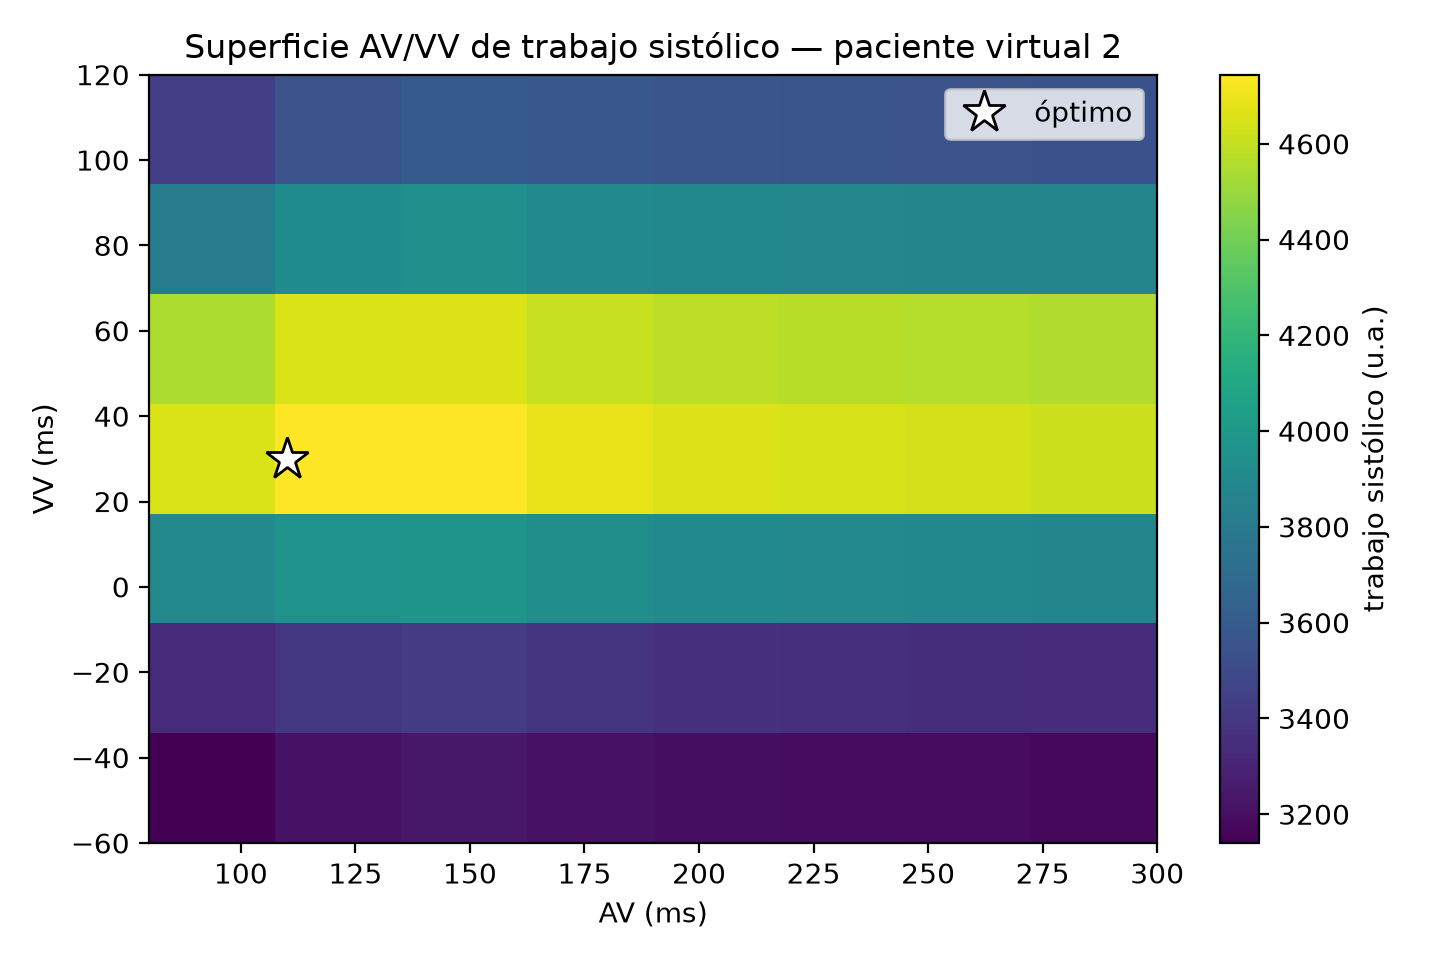
\includegraphics[width=0.78\linewidth]{response_surface.png}
\caption{Superficie de respuesta ilustrativa del trabajo sistólico AV/VV
simulado. El óptimo específico de cada paciente es el objetivo que los modelos de
ordenación intentan recuperar a partir de una señal de impedancia de un solo
latido.}
\label{fig:surface}
\end{figure}

\begin{figure}[htbp]
\centering
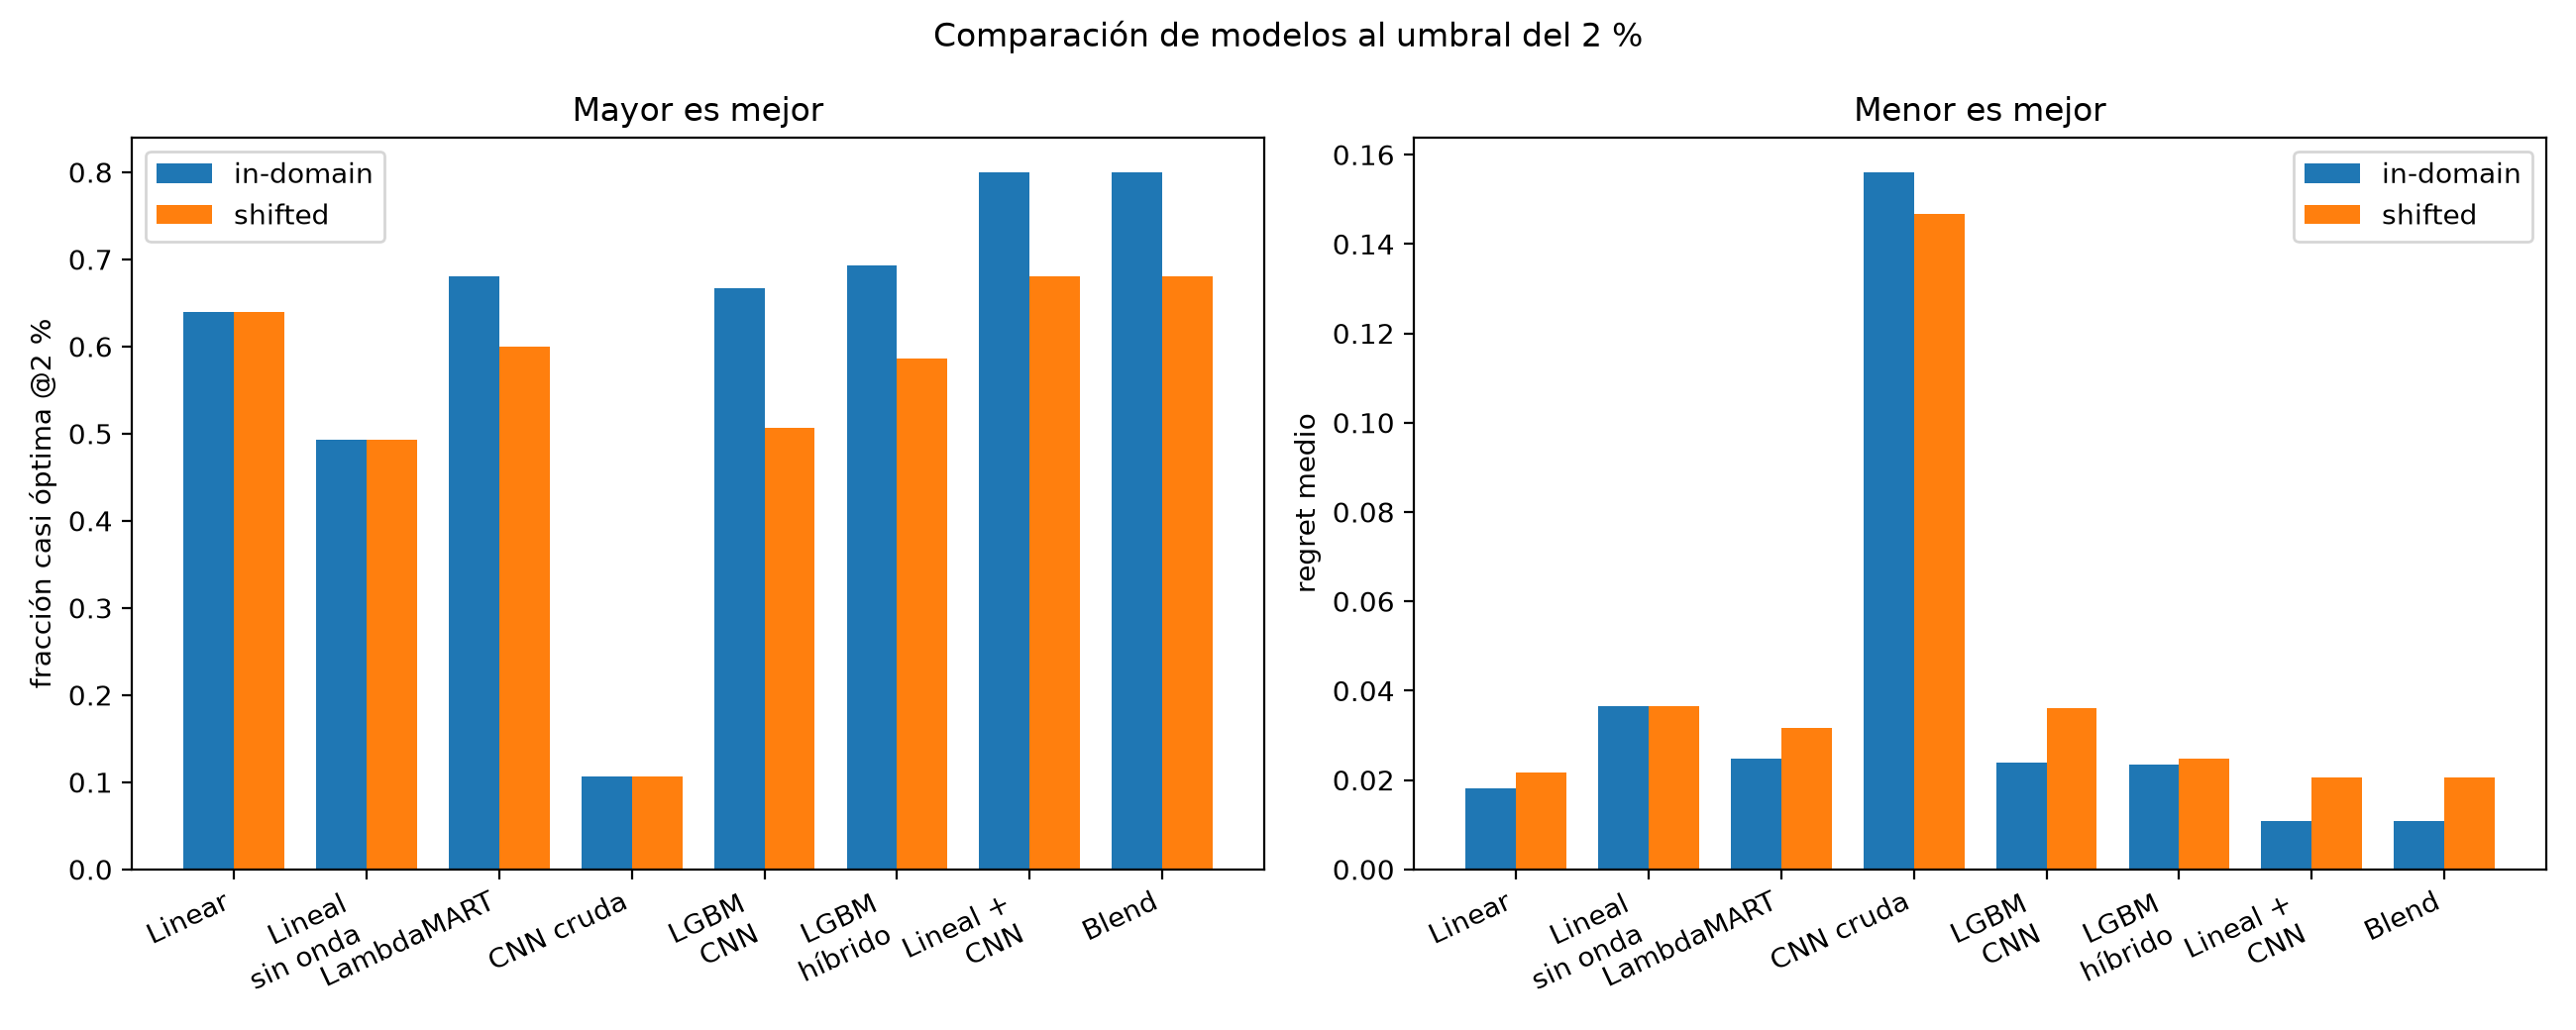
\includegraphics[width=0.95\linewidth]{model_comparison.png}
\caption{Fracción casi óptima y pérdida por modelo con el umbral del 2\,\%, en
dominio y bajo el desplazamiento sellado del sensor. Generado a partir de la
ejecución primaria reconciliada.}
\label{fig:models}
\end{figure}

\begin{figure}[htbp]
\centering
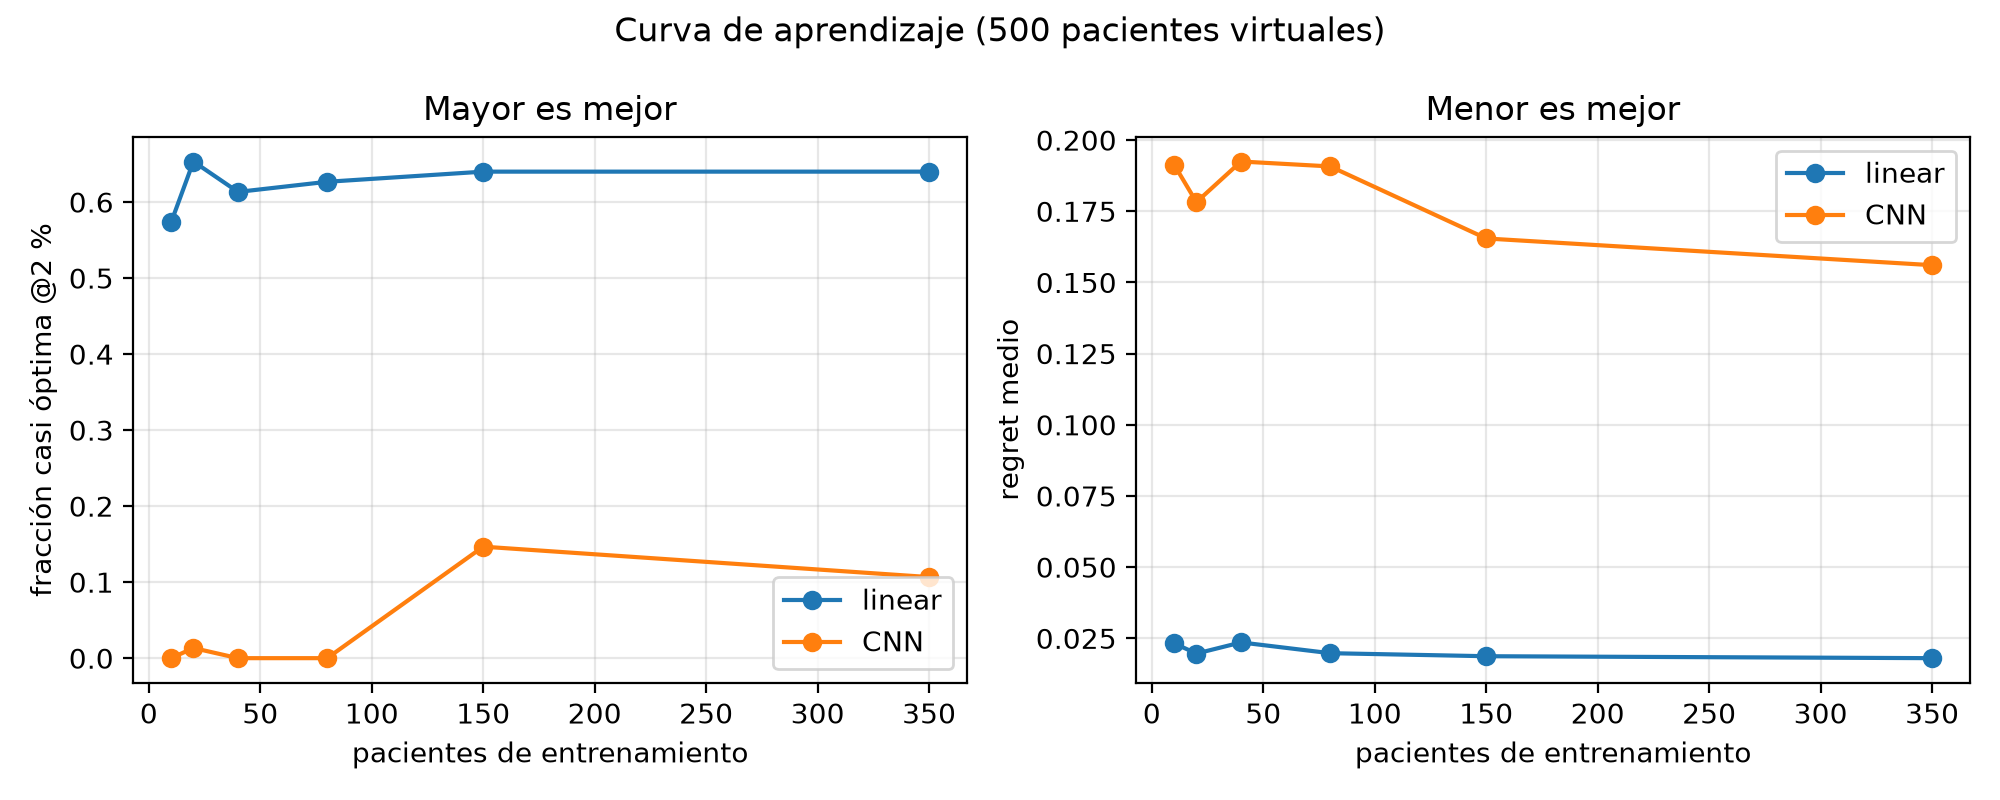
\includegraphics[width=0.75\linewidth]{learning_curve.png}
\caption{Curva de aprendizaje: fracción casi óptima y pérdida frente al número de
pacientes de entrenamiento. El modelo lineal se estabiliza entre 150 y 350
pacientes de entrenamiento.}
\label{fig:learning}
\end{figure}

\begin{figure}[htbp]
\centering
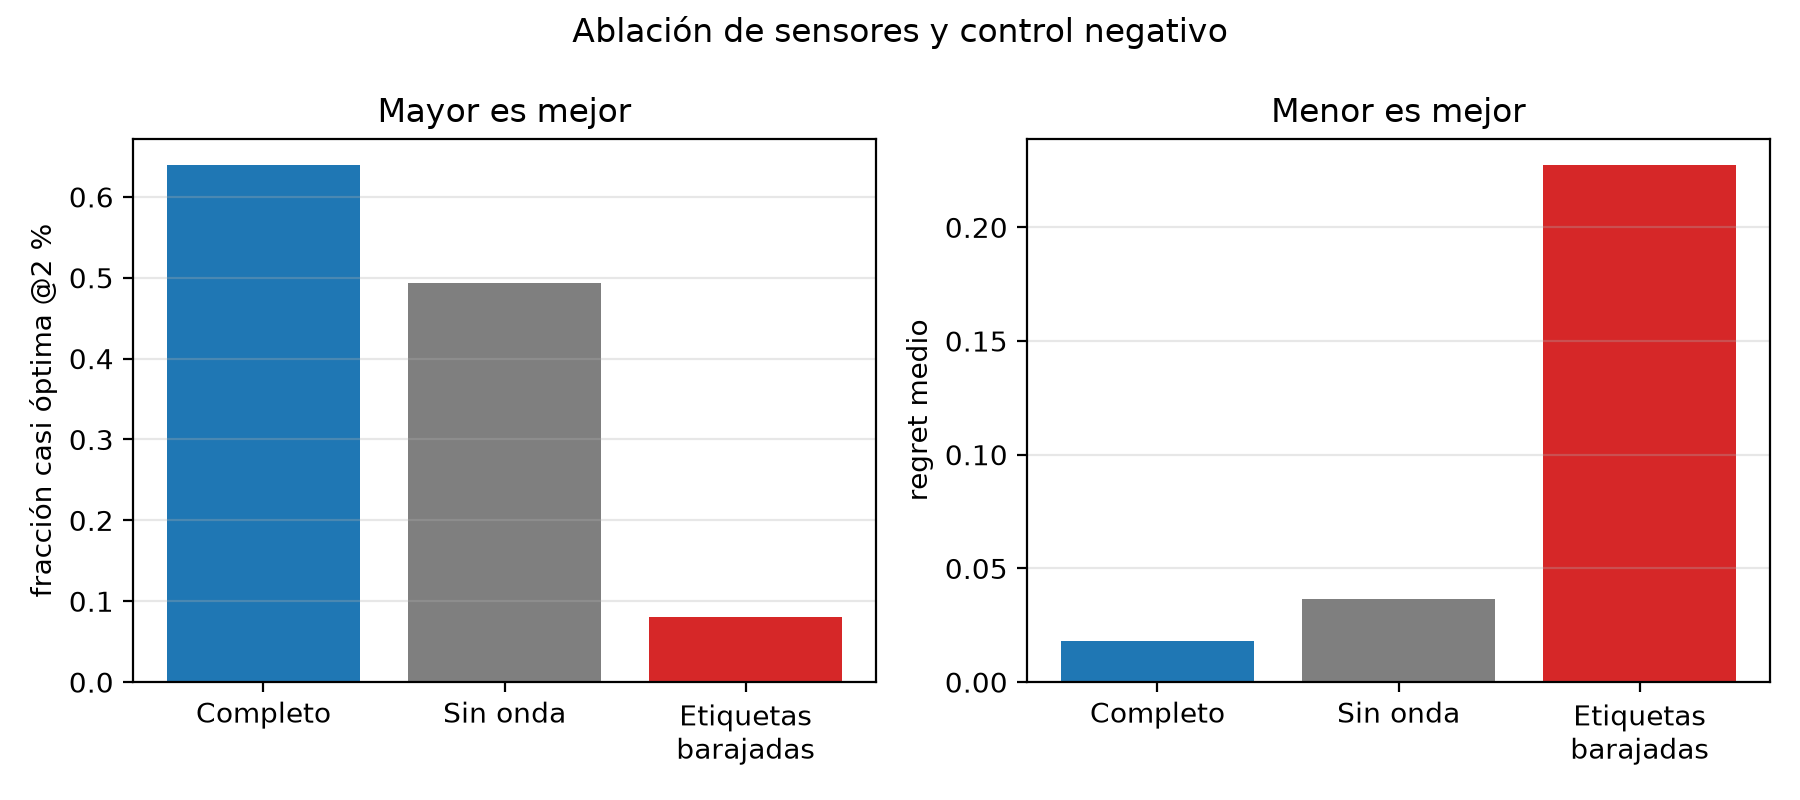
\includegraphics[width=0.85\linewidth]{ablations.png}
\caption{Ablaciones del sensor y control negativo. Eliminar las características
de la onda de impedancia devuelve el rendimiento al suelo sin onda (contexto y
programación).}
\label{fig:ablations}
\end{figure}

% -----------------------------------------------------------------------------
\bibliographystyle{plainnat}
\bibliography{references}
% -----------------------------------------------------------------------------

\end{document}
